\chapter{Mediciones de Aplicación} \label{ch:measurements}

% **************************** Define Graphics Path **************************
\ifpdf
    \graphicspath{{Chapter5/Figs/Raster/}{Chapter5/Figs/PDF/}{Chapter5/Figs/}}
\else
    \graphicspath{{Chapter5/Figs/Vector/}{Chapter5/Figs/}}
\fi

En este capítulo se realizan diferentes tipos de mediciones de aplicación. El mismo se encuentra dividido en dos secciones, la primera trata sobre ensayos aplicados en el simulador, para estudiar el efecto de la utilización de un objeto externo para la medición de la distancia entre el radar y el objeto a medir. La segunda sección resume los resultados obtenidos de las mediciones tomadas con el radar sobre un gabinete metálico y un corner reflector ante distintas distancias.


\section{Mediciones con Simulador}

En esta sección se realizan dos simulaciones para determinar la dependencia de la medición de los parámetros S del blanco iluminado con respecto a variaciones en la determinación de la distancia entre el objeto y el radar. 

En la figura \ref{fig:DistDependencySim} se observa que la distancia entre el mezclador y el blanco está determinada por la distancia real, $D$, sumada a un error, $\Delta D$. En la primer medición se tratará al error ($\Delta D$) como una variable conocida y configurable, en cambio, para la segunda medición se la tratará como una incertidumbre.

\begin{figure}[H]
  \centering
  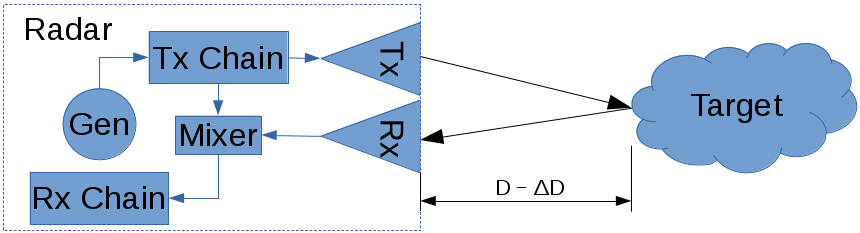
\includegraphics[width=12cm]{distanceDependency}
  \caption{Medición de propiedades del blanco ante diferentes diferencias de distancias.}
  \label{fig:DistDependencySim}
\end{figure}

Para disminuir el tiempo de procesamiento, se configuró el ancho de banda y la frecuencia central de la señal transmitida. Los valores son $\SI{300}{\kHz}$ y $\SI{2450}{\kHz}$ respectivamente. Dado que dichos parámetros son 3 órdenes de magnitud menores que la del radar, la resolución en rango simulada es 3 órdenes de magnitud mayor. Por lo tanto, las distancias a simular se incrementarán de la misma manera.


\subsection{Dependencia con distancia}

En esta sección se estudia la dependencia de la medición de un componente de la matriz de dispersión asociada al blanco iluminado con respecto a un error en la determinación de la distancia. Para ello, se simula que la distancia medida por el radar, $D_{medida}$, está determinada por la ecuación \ref{eq:distError}, siendo $D$ la distancia real entre el blanco y el radar y $\Delta D$ es un error conocido configurable.
\begin{equation} \label{eq:distError}
  D_{medida} = D - \Delta D
\end{equation}

\begin{table}[htb]
  \caption{Componente HH de la Matriz de dispersión del blanco a distintas distancias utilizando el simulador.}
  \centering
  \label{tab:simDeltaDist}
  \begin{tabular}{l *{4}{S[table-auto-round, table-format=1.1] S[table-auto-round, table-format=-3]}}
  \toprule
  \multirow{4}{1cm}{\textbf{Delta [m]}} & \multicolumn{8}{c}{\textbf{Distancia [m]}} \tabularnewline
  \cmidrule{2-9}
   & \multicolumn{2}{c}{30,760} & \multicolumn{2}{c}{35000} & \multicolumn{2}{c}{37760,1695} & \multicolumn{2}{c}{40000} \tabularnewline
  \cmidrule(r){2-3} \cmidrule(lr){4-5} \cmidrule(lr){6-7} \cmidrule(l){8-9}
   & {Gain} & {Phase} & {Gain} & {Phase} & {Gain} & {Phase} & {Gain} & {Phase} \tabularnewline
   & [$\si{\deci\bel}$] & [$\si{\degree}$] & [$\si{\deci\bel}$] & [$\si{\degree}$] & [$\si{\deci\bel}$] & [$\si{\degree}$] & [$\si{\deci\bel}$] & [$\si{\degree}$] \tabularnewline
  \midrule
  
  0 & 0.9974998783 & -0.8999873159 & 0.9970854521 & 5.0829022535 & 0.9974244573 & 0.0563536612 & 0.9991246271 & 1.1021289469 \tabularnewline

  5 & 0.996851467 & -28.5141663823 & 0.9965158111 & -22.5305974732 & 0.9968962677 & -27.5567038267 & 0.9986251585 & -26.5105696718 \tabularnewline

  10 & 0.9962033718 & -56.1283462497 & 0.9959464141 & -50.1440980009 & 0.9963682879 & -55.1697621157 & 0.9981258771 & -54.1232690916 \tabularnewline

  40 & 0.9923214343 & 138.1865577226 & 0.9925351551 & 144.1748820091 & 0.9932048122 & 139.1518713272 & 0.9951341194 & 140.2005175668 \tabularnewline

  100 & 0.984591606 & 166.8162791476 & 0.9857389337 & 172.8127555094 & 0.986900466 & 167.7950516932 & 0.9891707856 & 168.8480043635 \tabularnewline

  \bottomrule 
  \end{tabular}
\end{table}

La tabla \ref{tab:simDeltaDist} resume el componente HH de la matriz de dispersión obtenidos ante errores en la determinación de la distancia. La columna Delta indica el valor adoptado en la variable $\Delta D$ de la ecuación \ref{eq:distError}. Se puede observar que la variación que tiene $\Delta D$ en la determinación de la distancia en el resultado es despreciable para la ganancia, en cambio, para la fase, es totalmente determinante. Un acercamiento del blanco al radar de $\SI{5}{\meter}$ implica que la señal recorre $\SI{10}{\meter}$ menos, dado que la misma recorre el mismo camino dos veces. A su vez, independientemente de la distancia a la que está el blanco, un error igual a $\SI{5}{\meter}$ implica un desfase igual a $\SI{-28}{\degree}$. Este resultado es el esperado dado que la longitud de onda de la señal transmitida es aproximadamente $\SI{122}{\meter}$, por lo tanto un error de $\SI{12.2}{\meter}$ implica un desfase de $\SI{36}{\degree}$.

La figura \ref{fig:deltaDistSim} muestra de forma separada las mediciones de la ganancia y fase del blanco en las distancias $\SI{30760}{\meter}$, $\SI{35000}{\meter}$, $\SI{37760.1695}{\meter}$ y $\SI{40000}{\meter}$. Ĺos valores del gráfico de fase no coinciden con la tabla dado que, para enfatizar la linealidad de dicha variable con respecto a la distancia, se restaron $\SI{360}{\degree}$ cuando era necesario.
\begin{figure}[H]
  \centering
  \begin{subfigure}{0.49\textwidth}
    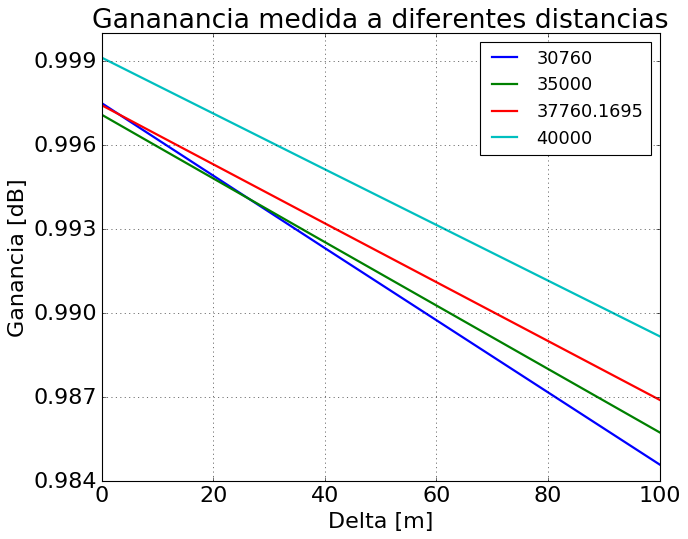
\includegraphics[width=7cm]{deltaDistGain}
    \caption{Ganancia}
  \end{subfigure}
  \begin{subfigure}{0.49\textwidth}
    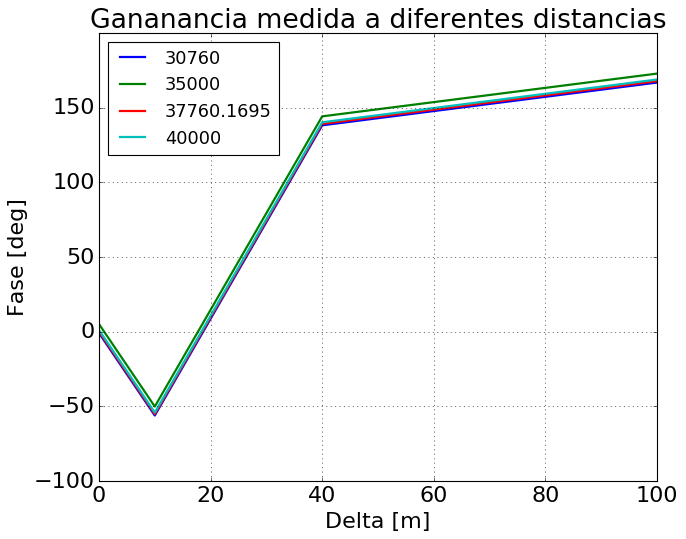
\includegraphics[width=7cm]{deltaDistPhase}
    \caption{Fase}
  \end{subfigure}
  \caption{Dependencia de la matriz de dispersión del blanco ante errores en la medición de la distancia al blanco.}
  \label{fig:deltaDistSim}
\end{figure}


\subsection{Incertidumbre en distancia}

En esta sección se introducen incertidumbres en la medición de la distancia buscando determinar cómo afecta a la medición de la matriz de dispersión del blanco iluminado. Dichas incertidumbres se las toma como ruido AWGN, por lo tanto poseen una distribución gaussiana con desvío estándar configurable y media igual a cero. La tabla \ref{tab:simIncertDist} resume los resultados obtenidos de la simulación de montecarlo con 1000 realizaciones.

\begin{table}[htb]
  \caption{Incertidumbre absoluta en el componente HH de la matriz de dispersión del blanco ante incertidumbre en la medición de distancia.}
  \centering
  \label{tab:simIncertDist}
  \begin{tabular}{l *{4}{S[table-auto-round, table-format=-1.3] S[table-auto-round, table-format=-3]}}
  \toprule
  \multirow{4}{1cm}{\textbf{Std [m]}} & \multicolumn{8}{c}{\textbf{Distancia [m]}} \tabularnewline
  \cmidrule{2-9}
   & \multicolumn{2}{c}{30760} & \multicolumn{2}{c}{35000} & \multicolumn{2}{c}{37760,1695} & \multicolumn{2}{c}{40000} \tabularnewline
  \cmidrule(r){2-3} \cmidrule(lr){4-5} \cmidrule(lr){6-7} \cmidrule(l){8-9}
   & {$\Delta Gain$} & {$\Delta Phase$} & {$\Delta Gain$} & {$\Delta Phase$} & {$\Delta Gain$} & {$\Delta Phase$} & {$\Delta Gain$} & {$\Delta Phase$} \tabularnewline
   & [$\si{\deci\bel}$] & [$\si{\degree}$] & [$\si{\deci\bel}$] & [$\si{\degree}$] & [$\si{\deci\bel}$] & [$\si{\degree}$] & [$\si{\deci\bel}$] & [$\si{\degree}$] \tabularnewline
  \midrule
  
  0 & 0.00 & 0.00 & 0.00 & 0.00 & 0.00 & 0.00 & 0.00 & 0.00 \tabularnewline

  5 & 0.000369507 & 15.7325843211 & 0.0003330912 & 16.1431290009 & 0.0002977873 & 15.5648756904 & 0.0002884168 & 15.9418570692 \tabularnewline

  10 & 0.0007337078 & 31.239336556 & 0.0006511433 & 31.5574962315 & 0.0006150956 & 32.1497974883 & 0.0005796089 & 32.0371315787 \tabularnewline

  40 & 0.0029849535 & 116.5644598149 & 0.002650077 & 116.673494049 & 0.0023426065 & 112.3447856255  & 0.0023238051 & 117.0437670382 \tabularnewline

  \bottomrule 
  \end{tabular}
\end{table}

Se puede observar que la variación en el resultado para la determinación de la ganancia es despreciable, en cambio, para la fase es totalmente determinante. Cabe destacar que la incertidumbre obtenida no depende de la distancia a la que se encuentra el blanco con respecto al radar.

La figura \ref{fig:incertDistSim} muestra la dependencia lineal entre la incertidumbre de la medición de la fase del blanco y el desvío estándar de la distancia al cual se encuentra. Se puede observar que, para cumplir con el requerimiento \ref{req:l1_phase}, y no tener una incertidumbre absoluta mayor a $\SI{30}{\degree}$, no se debe tener una incertidumbre en la distancia mayor a $\SI{8.33}{\meter}$.
\begin{figure}[H]
  \centering
  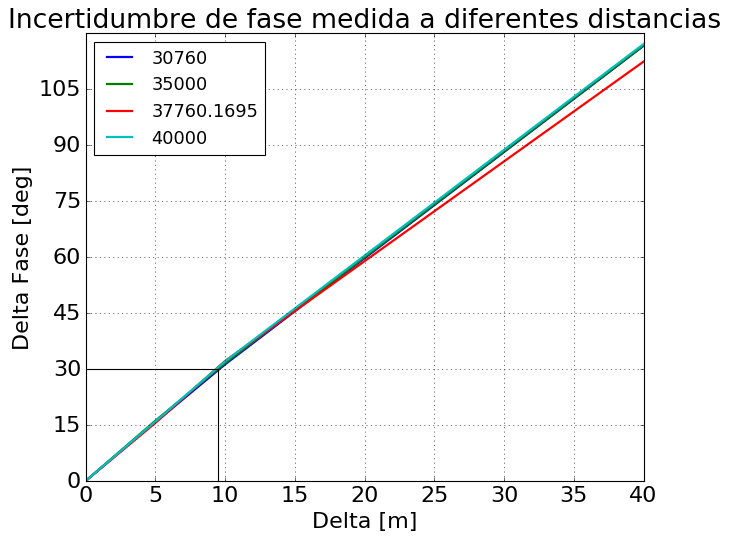
\includegraphics[width=7cm]{incertDistPhase}
  \caption{Medición de fase del blanco ante diferentes incertidumbres en distancias.}
  \label{fig:incertDistSim}
\end{figure}

\section{Mediciones con Radar}

En esta sección se realizan cuatro tipos de mediciones de aplicación con el radar utilizando diferentes blancos. En el primer caso se utiliza un gabinete rectangular frente a paneles absorbedores para disminuir los ecos en las paredes de la sala. En el segundo caso se estudia la dependencia de la estimación de la matriz de dispersión al tomar una distancia diferente a la real. Luego, en el tercer caso, se estudia el efecto de la presencia de incertidumbre en la distancia. Por último, en el cuarto caso, se mide un corner reflector.


\subsection{Medición de un gabinete metálico}

En esta sección se realizan diferentes mediciones variando la distancia entre el gabinete y el radar. Para disminuir el eco recibido de las paredes que se encuentran detrás del gabinete, se colocan paneles absorbedores. El objetivo de esta medición es la de determinar fuentes de incertidumbres que no se hayan tenido en cuenta previamente. Las imágenes de la figura \ref{fig:DistDependencySim2} muestran el ambiente de trabajo.
\begin{figure}[H]
  \centering
  \begin{subfigure}{0.59\textwidth}
    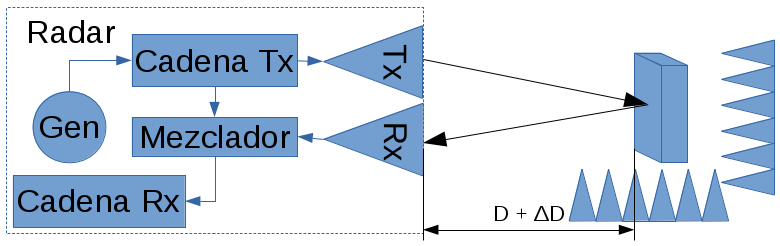
\includegraphics[width=9cm]{distanceDependencyRadar}
  \end{subfigure}
  \begin{subfigure}{0.39\textwidth}
    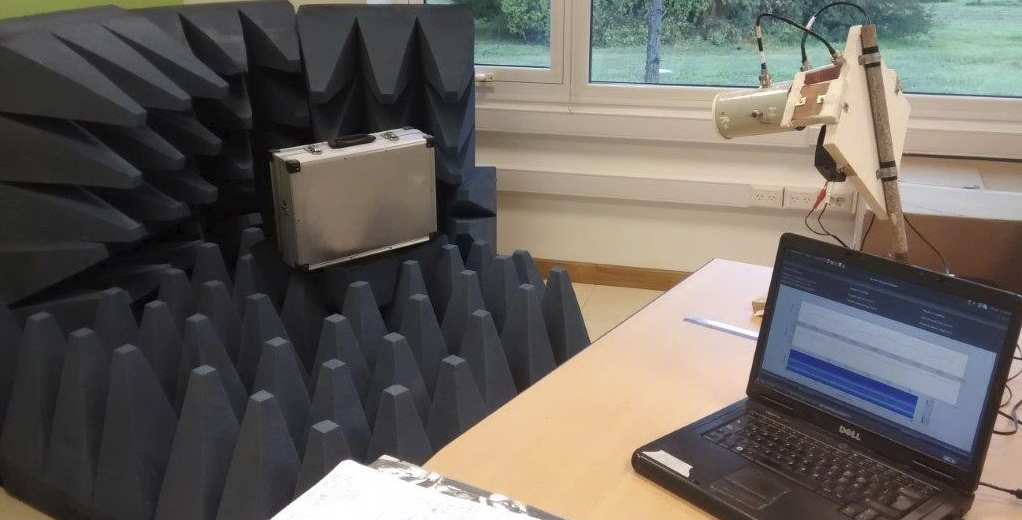
\includegraphics[width=6cm]{caseMeasurement}
  \end{subfigure}
  \caption{Medición de propiedades de un gabinete metálico ante diferentes distancias.}
  \label{fig:DistDependencySim2}
\end{figure}

La tabla \ref{tab:radarMeasurementResults} resume los resultados obtenidos. El error absoluto en las mediciones equivale a tres veces el desvío estándar, dado que se toma como hipótesis la de estar trabajando con una incertidumbre con distribución gaussiana.

\begin{table}[H]
  \caption{Matriz de dispersión del gabinete metálico medidos con el radar.}
  \centering
  \label{tab:radarMeasurementResults}
  \begin{tabular}{c c | *{2}{S[table-auto-round, table-format=1.3]} *{2}{S[table-auto-round, table-format=-2.2]} S[table-auto-round, table-format=-3] S[table-auto-round, table-format=2]}
  \toprule
  \textbf{Rango} & \textbf{Pol} & \textbf{Rango} & \textbf{$\Delta$Rango}  & \textbf{Gain} & \textbf{$\Delta$Gain} & \textbf{Phase} & \textbf{$\Delta$Phase} \tabularnewline

  [$\si{\meter}$] & & [$\si{\meter}$] & [$\si{\meter}$] & [$\si{\dB}$] & [$\si{\dB}$] & [$\si{\degree}$] & [$\si{\degree}$] \tabularnewline
  \midrule
  
  \multirow{4}{*}{1,32} & HH & 2.201 & 0.013 & 31.4539 & 0.0915 & 4.5 & 69.8 \tabularnewline
   & HV & 2.204 & 0.015 & 22.9796 & 0.1261 & -131.1 & 81.0 \tabularnewline
   & VH & 2.425 & 0.023 & 25.3829 & 0.2481 & -140.8 & 80.4 \tabularnewline
   & VV & 1.399 & 0.007 & 17.0184 & 0.1307 & 97.1 & 37.2 \tabularnewline

  \cmidrule{2-8}
  \multirow{4}{*}{1,56} & HH & 1.572 & 0.005 & 24.4271 & 0.0654 & -118.9 & 30.0 \tabularnewline
   & HV & 1.738 & 0.008 & 18.8475 & 0.0839 & -78.8 & 42.0 \tabularnewline
   & VH & 1.338 & 0.007 & 12.3065 & 0.0954 & 30.5 & 39.7 \tabularnewline
   & VV & 1.630 & 0.006 & 22.9165 & 0.1030 & -102.1 & 37.1 \tabularnewline

  \cmidrule{2-8}
  \multirow{4}{*}{1,71} & HH & 1.709 & 0.006 & 26.4757 & 0.0651 & 174.5 & 31.9 \tabularnewline
   & HV & 2.929 & 0.004 & 23.9049 & 0.0759 & -65.9 & 19.6 \tabularnewline
   & VH & 2.343 & 0.007 & 22.0027 & 0.0613 & -99.0 & 36.5 \tabularnewline
   & VV & 1.685 & 0.008 & 22.982 & 0.1295 & 58.9 & 49.5 \tabularnewline

  \cmidrule{2-8}
  \multirow{4}{*}{1,84} & HH & 1.994 & 0.006 & 28.0666 & 0.0532 & -90.1 & 33.6 \tabularnewline
   & HV & 1.224 & 0.007 & 5.9869 & 0.1663 & -61.1 & 40.2 \tabularnewline
   & VH & 2.258 & 0.006 & 18.3366 & 0.0649 & -1.3 & 31.9 \tabularnewline
   & VV & 2.072 & 0.003 & 26.4441 & 0.0632 & -73.7 & 22.2 \tabularnewline

  \cmidrule{2-8}
  \multirow{4}{*}{2,005} & HH & 2.364 & 0.008 & 30.0745 & 0.0695 & -190.8 & 43.1 \tabularnewline
   & HV & 3.896 & 0.013 & 25.8801 & 0.1221 & 10.7 & 71.8 \tabularnewline
   & VH & 2.259 & 0.006 & 18.1211 & 0.0513 & -7.8 & 35.5 \tabularnewline
   & VV & 2.108 & 0.005 & 24.5758 & 0.0572 & 15.0 & 28.8 \tabularnewline

  \bottomrule
  \end{tabular}
\end{table}

Analizando los resultados obtenidos en la tabla \ref{tab:radarMeasurementResults}, se pueden obtener las siguientes conclusiones:
\begin{description}
  \item[Determinación distancia] Se puede observar que se determina erróneamente la distancia al blanco. Esto se debe a que no se realizó una medición previa del clutter de la sala para substraer dicho efecto. En la figura \ref{fig:distanceError} se observa la FFT de la señal recibida, en la cual se indica que la potencia de la señal que se corresponde al eco del blanco es menor que la del propio clutter. De esta forma, se determina de una forma errónea la distancia al blanco.

  A su vez, se observa que sistemáticamente la ganancia para la polarización HH es mayor que para el resto. Dicho comportamiento se debe a que el crosstalk entre las antenas para dicha combinación de polarizaciones es la máxima medida, ver la sección \ref{ssc:sParameters}.

  \begin{figure}[H]
    \centering
    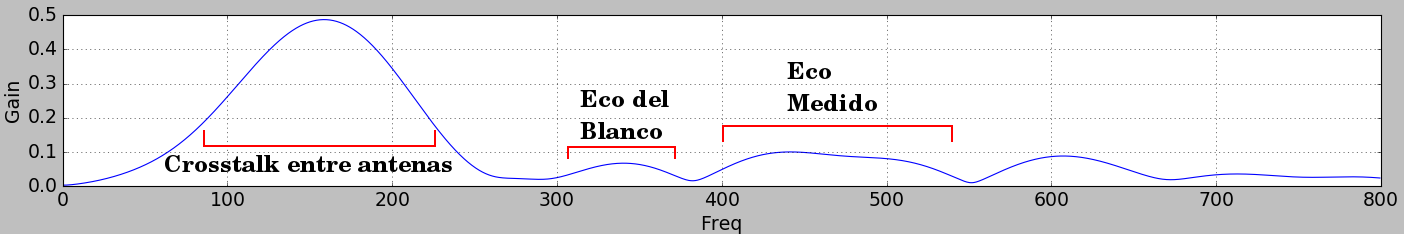
\includegraphics[width=15cm]{distanceError}
    \caption{FFT del eco recibido por el radar. Se observa que la potencia del eco recibido por el blanco es menor que el del clutter.}
    \label{fig:distanceError}
  \end{figure}

  \item[Determinación de Ganancia] Se puede observar que se determina erróneamente la relación de ganancia entre la señal incidente y reflejada del blanco. Esto se debe a tres causas principales. La primera se debe a que, como se mide de forma incorrecta la distancia al blanco, la atenuación real que impone el medio sobre la señal no es la calculada. La segunda está relacionada a que no se tomó en cuenta que el control del volumen de la computadora estaba en modo automático, por lo tanto entre ensayo y ensayo se modificó el nivel de la señal recibida, introduciendo un error grosero en dicha magnitud. La tercera se debe a que, como se puede observar en la figura \ref{fig:distanceError}, los niveles de potencia de la señal recibida son principalmente del clutter del ambiente. La mejor solución de este problema es la de realizar una medición previa del clutter sin blanco para realizar la resta de señales.

  \item[Determinación de Fase] Se puede observar que se determina erróneamente la relación de fase entre la señal incidente y reflejada del blanco. Esto es debe a dos causas principales. La primera se debe a que, como se mide de forma incorrecta la distancia al blanco, el desfase real que impone el medio sobre la señal no es la calculada. La segunda se debe a que, como no se eliminó el clutter de la señal, la medición resulta afectada.
\end{description}


\subsection{Dependencia con distancia}

En esta sección se estudia la dependencia de la medición de los parámetros S del blanco iluminado con respecto a un error en la determinación de la distancia. Para ello, se introduce en el procesador de la señal recibida del radar la distancia al blanco según la ecuación \ref{eq:distErrorRadar}. En donde $D$ es la distancia real entre el blanco y el radar y $\Delta D$ es un valor configurable. 
\begin{equation} \label{eq:distErrorRadar}
  D_{medida} = D - \Delta D
\end{equation}

\begin{table}[H]
  \caption{Componente HH de la matriz de dispersión del blanco a distintas distancias utilizando el radar.}
  \centering
  \label{tab:simDeltaDistRadar}
  \begin{tabular}{l *{3}{S[table-auto-round, table-format=-1.2] S[table-auto-round, table-format=-3]}}
  \toprule
  \multirow{4}{1cm}{\textbf{Delta [$\si{\milli\meter}$]}} & \multicolumn{6}{c}{\textbf{Distancia [$\si{\meter}$]}} \tabularnewline
  \cmidrule{2-7}
   & \multicolumn{2}{c}{2,201} & \multicolumn{2}{c}{2,229} & \multicolumn{2}{c}{2,255} \tabularnewline
  \cmidrule(r){2-3} \cmidrule(lr){4-5} \cmidrule(l){6-7}
   & {Gain} & {Phase} & {Gain} & {Phase} & {Gain} & {Phase} \tabularnewline
   & [$\si{\dB}$] & [$\si{\degree}$] & [$\si{\dB}$] & [$\si{\degree}$] & [$\si{\dB}$] & [$\si{\degree}$] \tabularnewline
  \midrule
  
  0 & -1.8092 & 147.7 & -1.8941 & 133.2 & -1.4372 & 152.1 \tabularnewline

  5 & -1.8570 & 174.8 & -1.9362 & 161.4 & -1.4903 & 179.8 \tabularnewline

  10 & -1.8940 & 202 & -1.9772 & 188.0 & -1.5177 & 207.0 \tabularnewline

  15 & -1.9243 & 229.5 & -2.0172 & 215.5 & -1.5622 & 234.4 \tabularnewline

  \bottomrule 
  \end{tabular}
\end{table}
La tabla \ref{tab:simDeltaDistRadar} resume los componentes HH de la matriz de dispersión obtenidos ante errores en la determinación de la distancia. La columna Delta indica el valor adoptado en la variable $\Delta D$ de la ecuación \ref{eq:distErrorRadar}. Se puede observar que la variación en el resultado para la determinación de la ganancia resulta despreciable dado que al haber $\SI{15}{\milli\meter}$ de diferencia la medición disminuyó en $\SI{0.12}{\dB}$ y para el caso de la fase es totalmente determinante. Cabe destacar que un error en la medición de distancia de $\SI{5}{\milli\meter}$ implica que la señal recorre $\SI{10}{\milli\meter}$ menos, dado que la misma recorre el mismo camino dos veces. A su vez, independientemente de la distancia a la que está el blanco, un error igual a $\SI{5}{\milli\meter}$ implica un desfase igual a $\SI{27.6}{\degree}$. Este resultado es el esperado dado que la longitud de onda de la señal transmitida es aproximadamente $\SI{122}{\milli\meter}$, por lo tanto un error de $\SI{12.2}{\meter}$ implica un desfase de $\SI{36}{\degree}$.

\begin{figure}[H]
  \centering
  \begin{subfigure}{0.49\textwidth}
    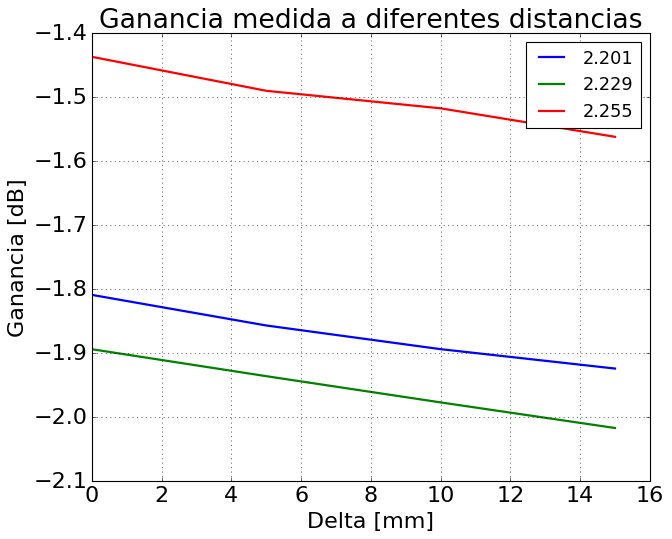
\includegraphics[width=7cm]{deltaDistGainRadar}
    \caption{Ganancia}
  \end{subfigure}
  \begin{subfigure}{0.49\textwidth}
    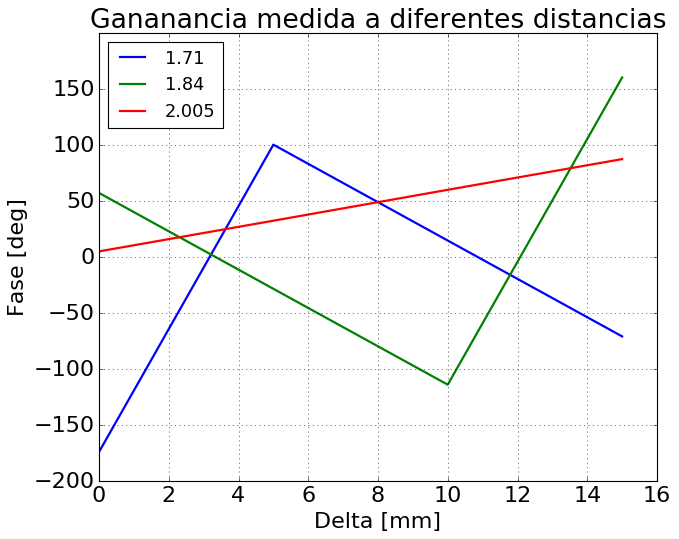
\includegraphics[width=7cm]{deltaDistPhaseRadar}
    \caption{Fase}
  \end{subfigure}
  \caption{Parámetros S del blanco a distintas distancias.}
  \label{fig:deltaDistRadar}
\end{figure}
La figura \ref{fig:deltaDistRadar} muestra de forma separada las mediciones de la ganancia y fase del blanco en las distancias $\SI{2.201}{\meter}$, $\SI{2.229}{\meter}$ y $\SI{2.255}{\meter}$. Se puede observar que tanto la ganancia como el desfase son del mismo orden para cada distancia.


\subsection{Incertidumbre en Distancia} \label{ssc:distIncert}

En esta sección se estudia la dependencia de las incertidumbres obtenidas de los parámetros S del blanco iluminado con respecto a la incertidumbre de la distancia. Para ello se analiza la misma adquisición dos veces, la primera introduciendo la distancia en el programa, y en la segunda utilizando el rango determinado por el radar.

La tabla \ref{tab:radarDistIncert} está dividida en dos partes. A la izquierda de la misma se muestran las incertidumbres obtenidas sin incertidumbre en distancia. En cambio, a la derecha, se muestran dichos resultados con incertidumbre en distancia.

\begin{table}[H]
  \caption{Dependencia de incertidumbre de los parámetros S medidos ante incertidumbre en la distancia.}
  \centering
  \label{tab:radarDistIncert}
  \begin{tabular}{c c | S[table-auto-round, table-format=1.1] S[table-auto-round, table-format=2] || *{2}{S[table-auto-round, table-format=-2.2]} S[table-auto-round, table-format=1.1] S[table-auto-round, table-format=3]}
  \toprule
  \textbf{Rango} & \textbf{Pol} & \textbf{$\Delta$Gain} & \textbf{$\Delta$Phase} & \textbf{Rango} & \textbf{$\Delta$Rango}  & \textbf{$\Delta$Gain} & \textbf{$\Delta$Phase} \tabularnewline

  [$\si{\meter}$] & & [$\si{\dB}$] & [$\si{\degree}$] & [$\si{\meter}$] & [$\si{\meter}$] & [$\si{\dB}$] & [$\si{\degree}$] \tabularnewline
  \midrule

  \multirow{4}{*}{2,201} & HH & 0.4531 & 9.1 & 2.201 & 0.011 & 0.4921 & 56.3 \tabularnewline
   & HV & 1.5631 & 13.9 & 2.247 & 0.026 & 1.5951 & 163.6 \tabularnewline
   & VH & 2.1342 & 87.1 & 2.288 & 0.036 & 2.205 & 204.8 \tabularnewline
   & VV & 0.3614 & 7.3 & 2.195 & 0.014 & 0.3789 & 82.1 \tabularnewline

  \bottomrule
  \end{tabular}
\end{table}

Analizando los resultados de la tabla \ref{tab:radarDistIncert}, se puede llegar a la conclusión que la incertidumbre en la ganancia no se ve afectada ante la eliminación de la incertidumbre en la distancia. En cambio, se puede observar una fuerte dependencia de la incertidumbre de fase con respecto a la incertidumbre de distancia.


\subsection{Medición de un Corner Reflector}

Para esta experiencia se construye un corner reflector triangular de $\SI{50}{\centi\meter}$ de lado, ver figura \ref{fig:corner}. El máximo RCS que se puede obtener, siguiendo la ecuación \ref{eq:theoreticalRcs}, es igual a $\SI{12.43}{\dB}$.
\begin{figure}[H]
  \centering
  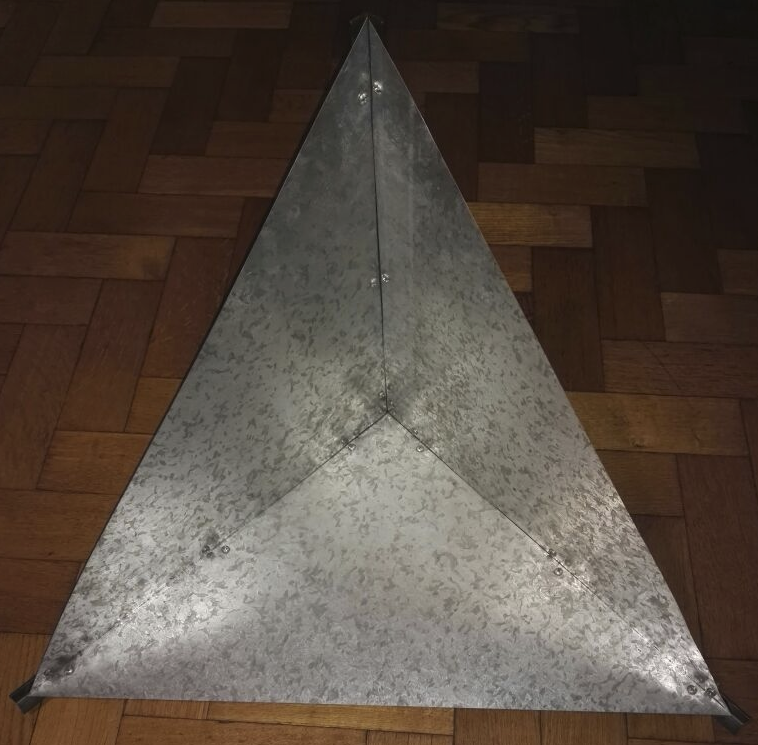
\includegraphics[width=6cm]{cornerReflector}
  \caption{Corner reflector construido de $\SI{50}{\centi\meter}$ de lado para realizar las mediciones.}
  \label{fig:corner}
\end{figure}

La disposición del radar y del corner reflector en la sala se muestra en las imágenes de la  figura \ref{fig:cornerMeasurement}. Se puede determinar que el ángulo de incidencia con respecto a la horizontal resulta del orden de $\SI{24}{\degree}$. Por lo tanto, se espera una disminución de $\SI{3}{\dB}$, la cual se determina en la figura \ref{fig:cornerRel}. A su vez, en la figura \ref{fig:cornerErrors} se muestra cómo el RCS resulta afectado ante la pérdida de ortogonalidad entre las caras del corner. Se espera que haya una pérdida extra del orden de los $\SI{10}{\dB}$.
\begin{figure}
  \centering
  \begin{subfigure}{0.54\textwidth}
    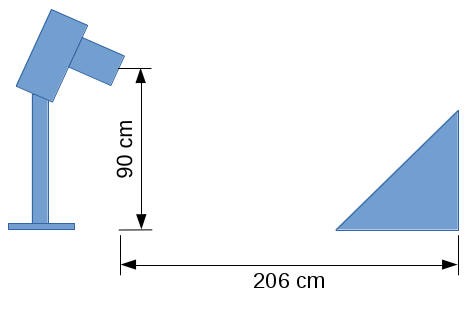
\includegraphics[width=8cm]{cornerMeasurementScheme}
  \end{subfigure}
  \begin{subfigure}{0.44\textwidth}
    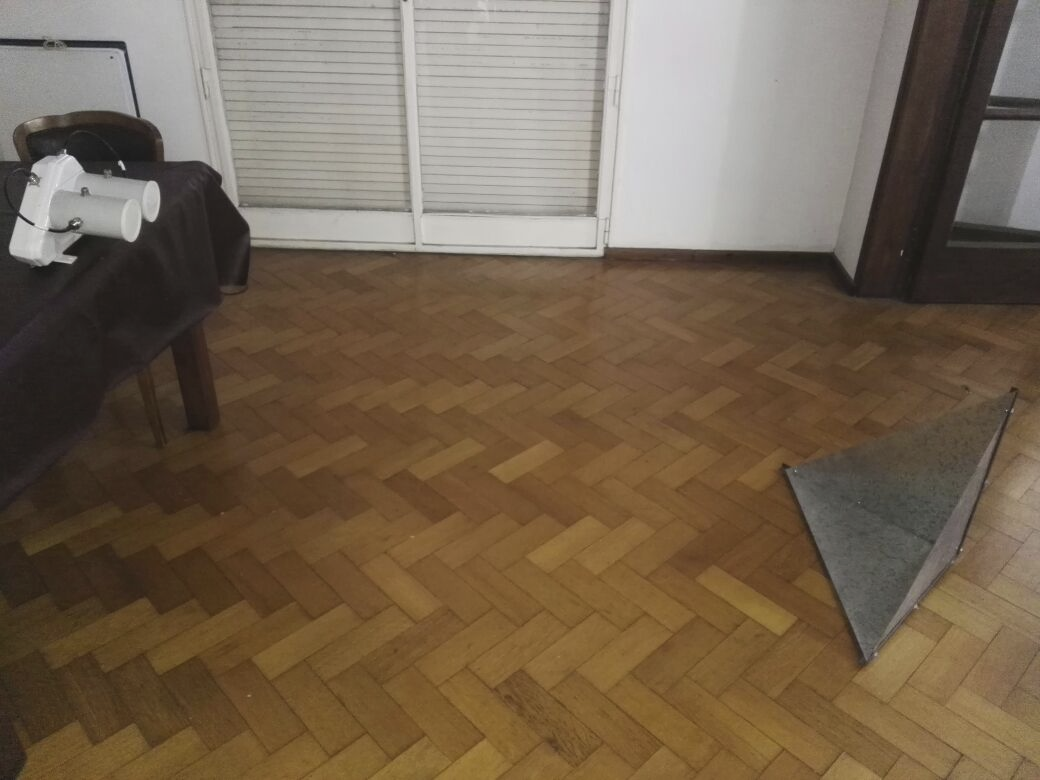
\includegraphics[width=6.5cm]{cornerMeasurement}
  \end{subfigure}
  \caption{Medición de propiedades del corner reflector ante diferentes distancias.}
  \label{fig:cornerMeasurement}
\end{figure}
La tabla \ref{tab:cornerMeasurementResults} resume los resultados obtenidos. El error absoluto en las mediciones equivale a tres veces el desvío estándar, dado que se toma como hipótesis la de estar trabajando con una incertidumbre con distribución gaussiana. Dado que se obtienen mejores resultados de fase midiendo la distancia del radar al blanco de forma externa, ver la sección \ref{ssc:distIncert} Incertidumbre en Distancia, se utiliza una cinta métrica para dichas mediciones. Por último, las mediciones se realizaron en dos etapas, primero se mide el clutter, adquisición sin el blanco y luego con el blanco, restando el clutter medido previamente.

\begin{table}[H]
  \caption{Parámetros de dispersión del corner reflector medidos con el radar.}
  \centering
  \label{tab:cornerMeasurementResults}
  \begin{tabular}{c c | S[table-auto-round, table-format=1.2] S[table-auto-round, table-format=1.2] S[table-auto-round, table-format=-2.2] S[table-auto-round, table-format=1.2] S[table-auto-round, table-format=-3] S[table-auto-round, table-format=2]}
  \toprule
  \textbf{Rango} & \textbf{Pol} & \textbf{Rango} & \textbf{$\Delta$Rango}  & \textbf{Gain} & \textbf{$\Delta$Gain} & \textbf{Phase} & \textbf{$\Delta$Phase} \tabularnewline

  [$\si{\meter}$] & & [$\si{\meter}$] & [$\si{\meter}$] & [$\si{\dB}$] & [$\si{\dB}$] & [$\si{\degree}$] & [$\si{\degree}$] \tabularnewline
  \midrule

  \multirow{4}{*}{2,201} & HH & 2.201 & 0.011 & -1.3969 & 0.4531 & -7.8 & 9.1 \tabularnewline
   & HV & 2.247 & 0.026 & -14.0225 & 1.5631 & -73.1 & 13.9 \tabularnewline
   & VH & 2.288 & 0.036 & -14.1252 & 2.1342 & -92.4 & 87.1 \tabularnewline
   & VV & 2.195 & 0.014 & -1.8092 & 0.3614 & 147.7 & 7.3 \tabularnewline

  \cmidrule{2-8}
  \multirow{4}{*}{2,229} & HH & 2.223 & 0.017 & -1.2961 & 0.3128 & -11.0 & 9.3 \tabularnewline
   & HV & 2.313 & 0.041 & -13.3133 & 1.5806 & -71.5 & 14.0 \tabularnewline
   & VH & 2.317 & 0.038 & -14.7132 & 2.3655 & -93.3 & 87.3 \tabularnewline
   & VV & 2.246 & 0.023 & -1.8941 & 0.2935 & 133.2 & 12.3 \tabularnewline

  \cmidrule{2-8}
  \multirow{4}{*}{2,255} & HH & 2.26 & 0.01 & -1.6825 & 0.4407 & -4.0 & 5.2 \tabularnewline
   & HV & 2.305 & 0.038 & -14.2542 & 1.2031 & -59.7 & 18.3 \tabularnewline
   & VH & 2.359 & 0.049 & -13.4975 & 1.8296 & -95.4 & 33.8 \tabularnewline
   & VV & 2.245 & 0.019 & -1.4372 & 0.3531 & 152.1 & 7.8 \tabularnewline

  \cmidrule{2-8}
  \multirow{4}{*}{2,285} & HH & 2.272 & 0.021 & -1.9684 & 0.4278 & -3.23 & 9.9 \tabularnewline
   & HV & 2.398 & 0.039 & -14.3538 & 1.1613 & -83.6 & 16.9 \tabularnewline
   & VH & 2.379 & 0.052 & -14.1736 & 1.5638 & -95.2 & 60.2 \tabularnewline
   & VV & 2.287 & 0.023 & -1.6621 & 0.3498 & 177.4 & 12.4 \tabularnewline

  \bottomrule
  \end{tabular}
\end{table}

Las figuras \ref{fig:measuredDistCorner}, \ref{fig:measuredGainCorner} y \ref{fig:measuredPhaseCorner} muestran las distancias, ganancias y desfases esperados y medidos por le radar asociados a sus respectivas incertidumbres con respecto a las distintas distancias medidas de forma externa. Se puede concluir lo siguiente:
\begin{figure}[H]
  \centering
  \begin{subfigure}{0.49\textwidth}
    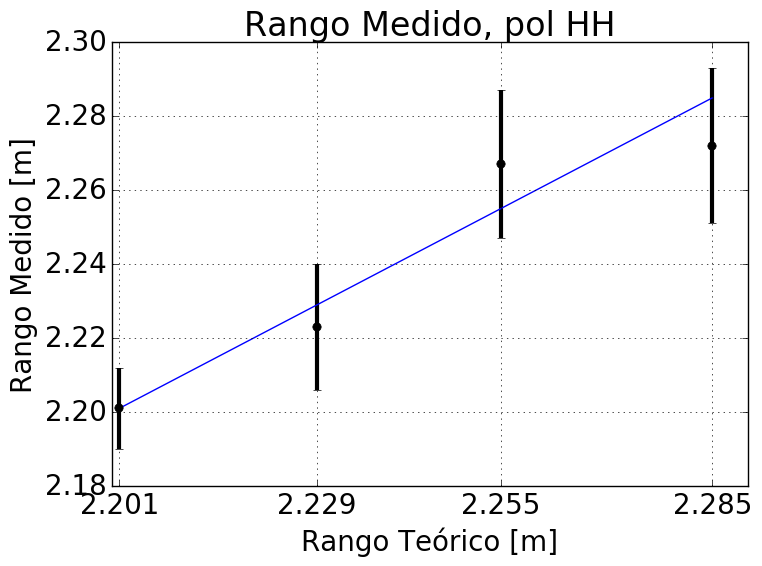
\includegraphics[width=6cm]{measuredCornerRangeHH}
  \end{subfigure}
  \begin{subfigure}{0.49\textwidth}
    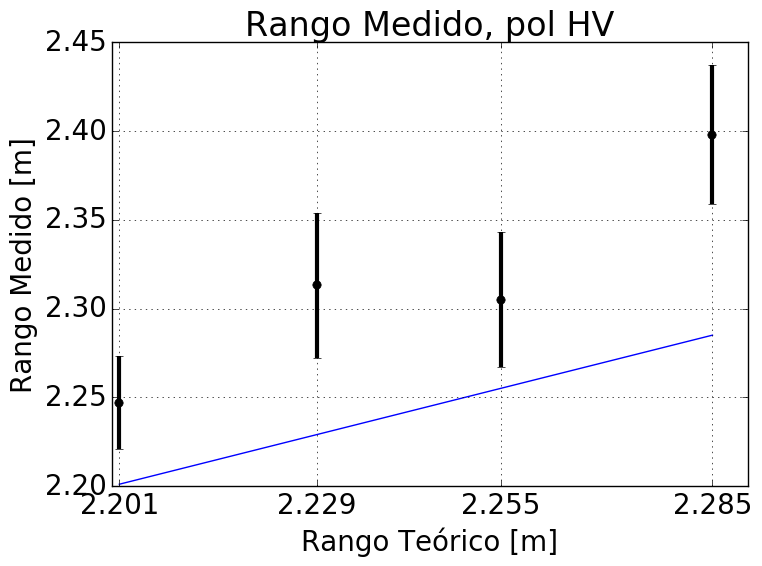
\includegraphics[width=6cm]{measuredCornerRangeHV}
  \end{subfigure}

  \begin{subfigure}{0.49\textwidth}
    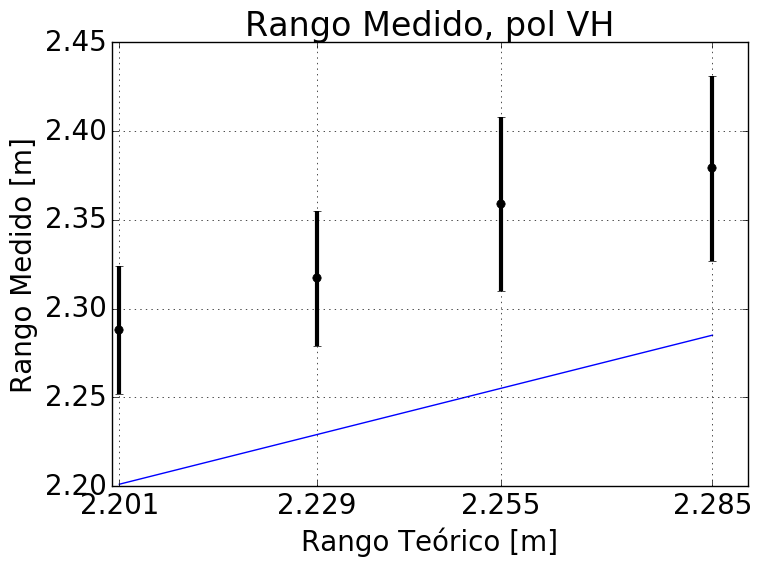
\includegraphics[width=6cm]{measuredCornerRangeVH}
  \end{subfigure}
  \begin{subfigure}{0.49\textwidth}
    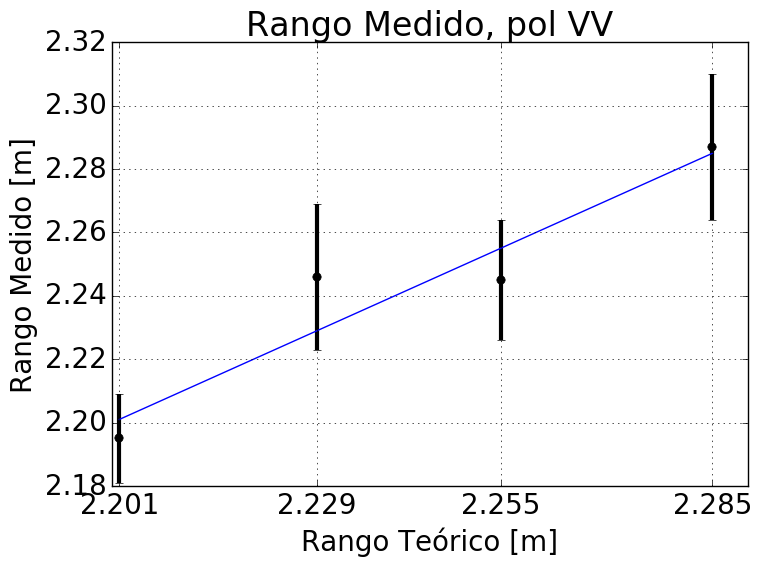
\includegraphics[width=6cm]{measuredCornerRangeVV}
  \end{subfigure}
  \caption{Distancia medida con su incertidumbre por el radar con respecto a la distancia medida con una cinta métrica.}
  \label{fig:measuredDistCorner}
\end{figure}
\begin{figure}[H]
  \centering
  \begin{subfigure}{0.49\textwidth}
    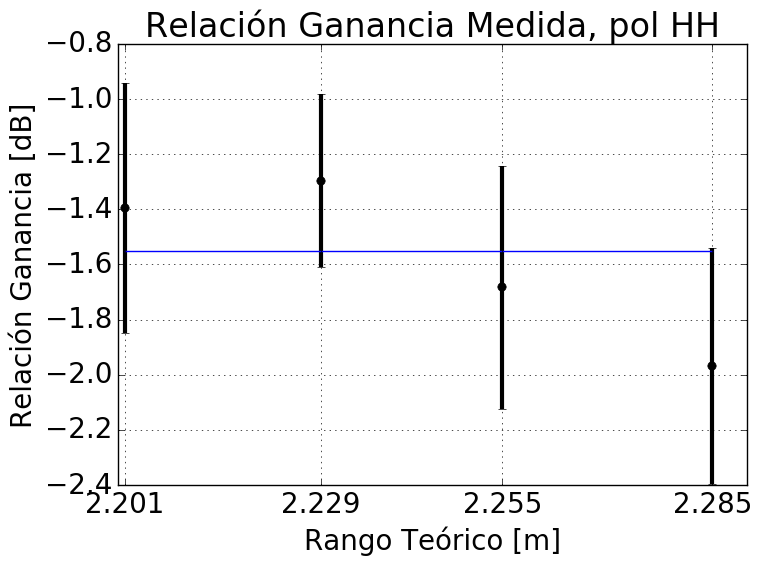
\includegraphics[width=6cm]{measuredCornerGainHH}
  \end{subfigure}
  \begin{subfigure}{0.49\textwidth}
    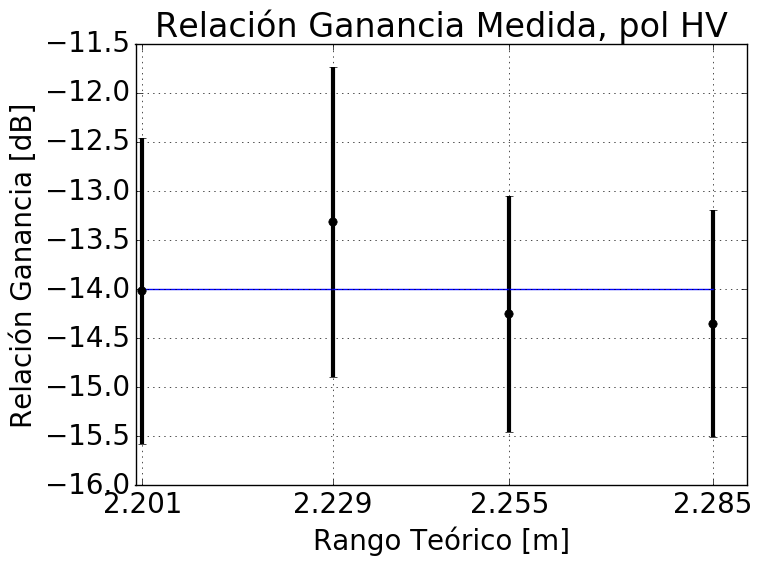
\includegraphics[width=6cm]{measuredCornerGainHV}
  \end{subfigure}

  \begin{subfigure}{0.49\textwidth}
    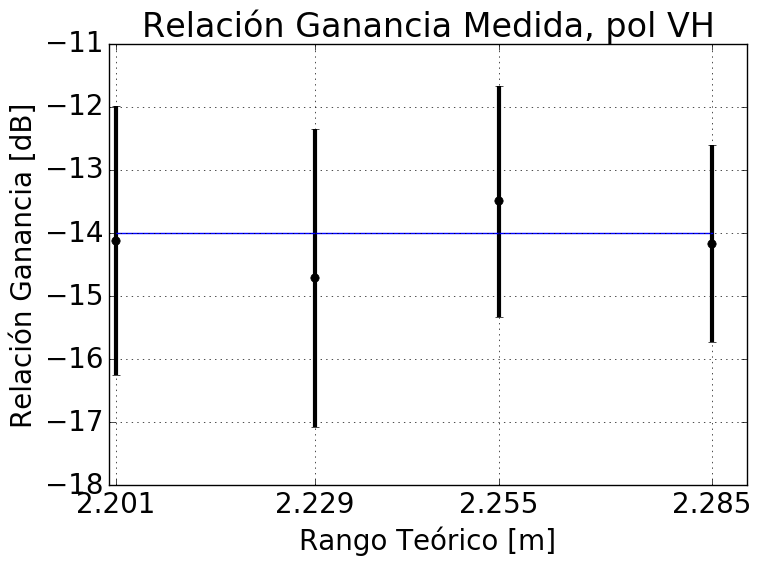
\includegraphics[width=6cm]{measuredCornerGainVH}
  \end{subfigure}
  \begin{subfigure}{0.49\textwidth}
    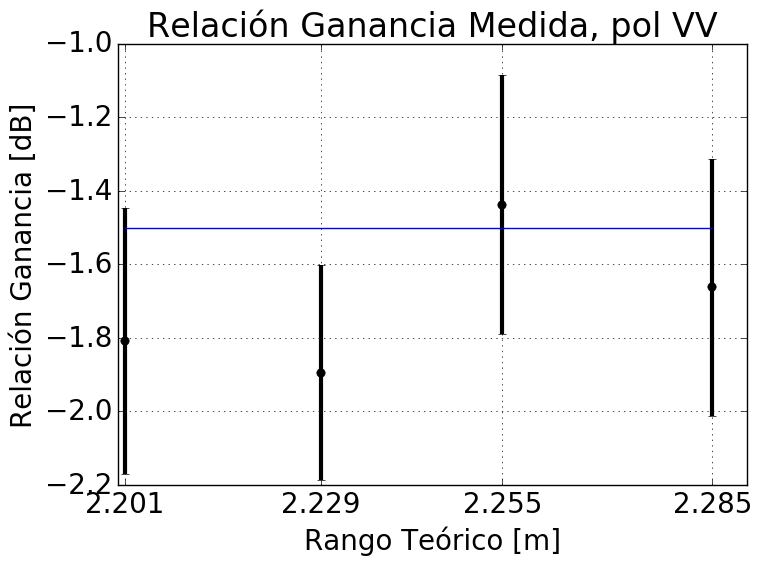
\includegraphics[width=6cm]{measuredCornerGainVV}
  \end{subfigure}
  \caption{Ganancia medida del blanco con su incertidumbre por el radar con respecto a la distancia medida con una cinta métrica.}
  \label{fig:measuredGainCorner}
\end{figure}
\begin{figure}[H]
  \centering
  \begin{subfigure}{0.49\textwidth}
    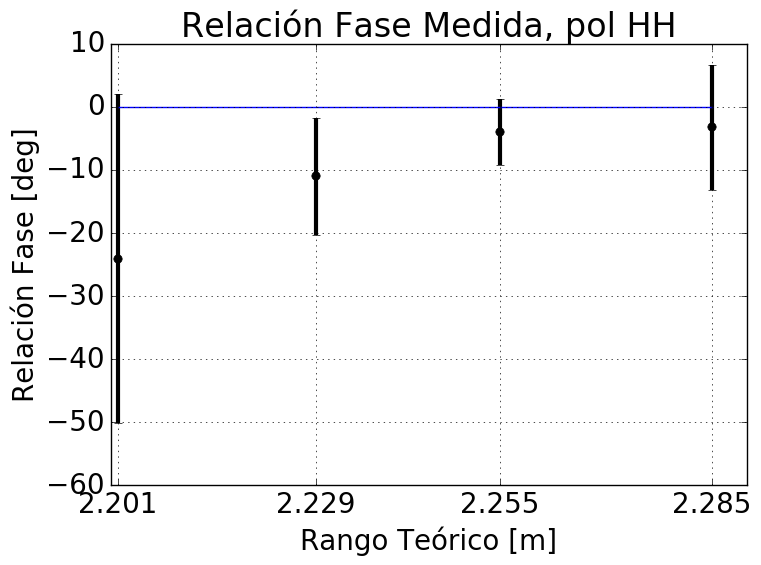
\includegraphics[width=6cm]{measuredCornerPhaseHH}
  \end{subfigure}
  \begin{subfigure}{0.49\textwidth}
    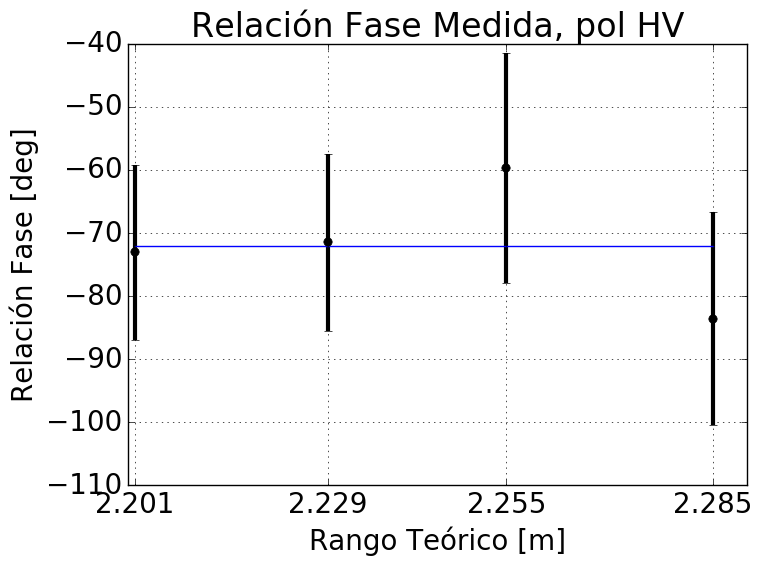
\includegraphics[width=6cm]{measuredCornerPhaseHV}
  \end{subfigure}

  \begin{subfigure}{0.49\textwidth}
    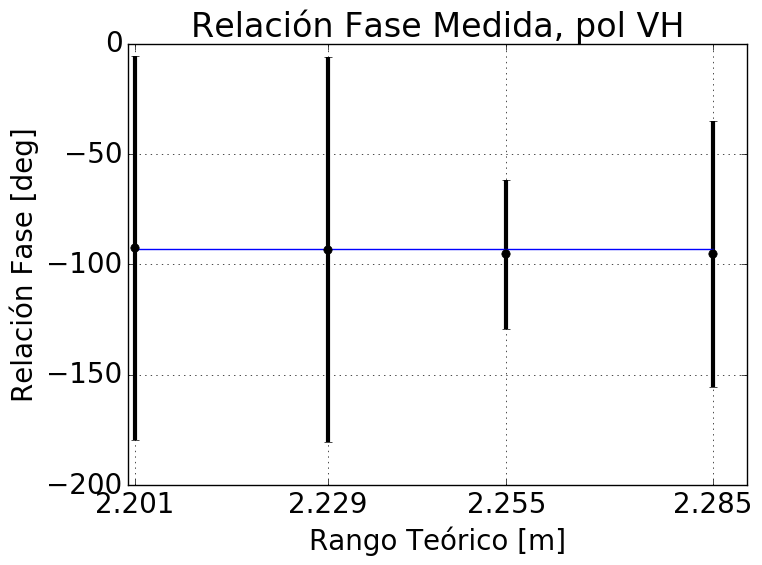
\includegraphics[width=6cm]{measuredCornerPhaseVH}
  \end{subfigure}
  \begin{subfigure}{0.49\textwidth}
    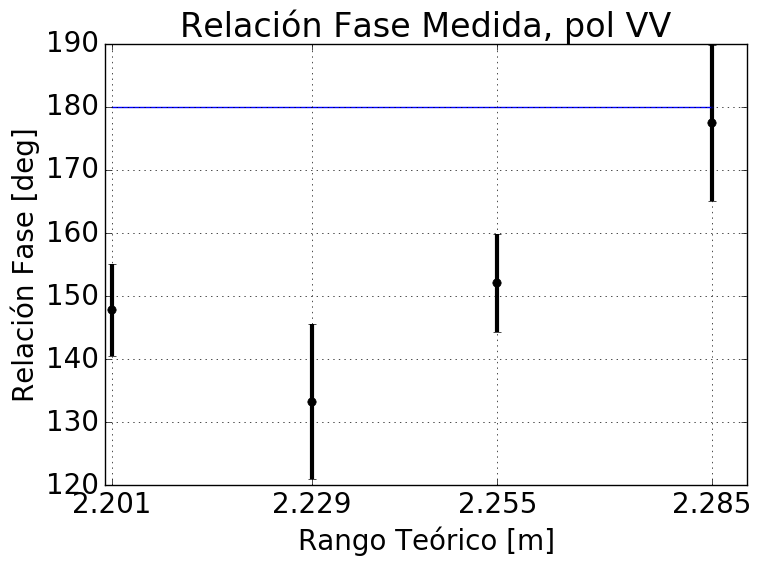
\includegraphics[width=6cm]{measuredCornerPhaseVV}
  \end{subfigure}
  \caption{Fase medida del blanco con su incertidumbre por el radar con respecto a la distancia medida con una cinta métrica.}
  \label{fig:measuredPhaseCorner}
\end{figure}


\begin{description}
  \item[Determinación de distancia] En la figura \ref{fig:measuredDistCorner} se puede observar que el radar determina correctamente la distancia al blanco para las adquisiciones co-polares. En cambio, como el corner posee un alto rechazo para adquisiciones cross-polares, el radar detecta la presencia de otro cuerpo de la sala en que se realizaron las mediciones. Hay algunas adquisiciones co-polares en donde la distancia indicada por el radar es un par de centímetros mayor al ideal, esto se debe a que entre adquisiciones el blanco fue removido y vuelto a colocar sin volver a medir que el mismo quede exactamente en la misma posición. En la figura \ref{fig:correctDistance} se muestra la FFT de la señal recibida con el blanco luego de haber eliminado el clutter.

  \begin{figure}[H]
    \centering
    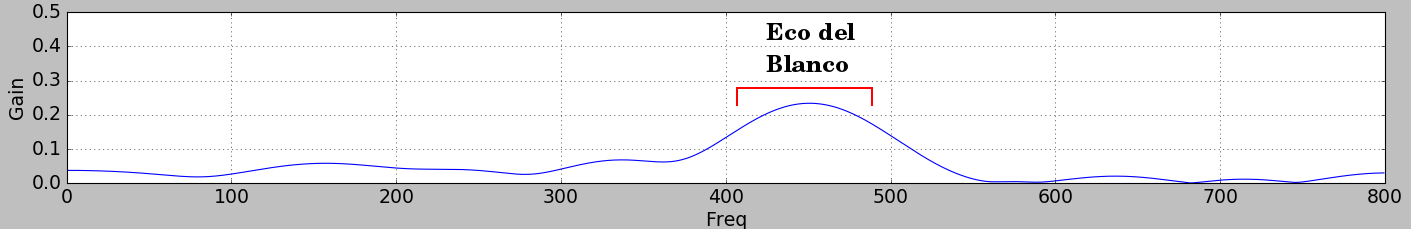
\includegraphics[width=15cm]{correctDistance}
    \caption{FFT del eco recibido por el radar. Se observa que la potencia del eco recibido por el blanco es mayor que el del clutter.}
    \label{fig:correctDistance}
  \end{figure}

  \item[Determinación de Ganancia] En la figura \ref{fig:measuredGainCorner} se puede observar que el radar detecta correctamente las ganancias del corner reflector. Se aprecia una disminución de $\SI{14}{\dB}$ para adquisiciones cross-polares con respecto a las co-polares. A su vez, se puede apreciar que las adquisiciones co-polares poseen una ganancia del orden de los $\SI{-1.5}{\dB}$ con una incertidumbre absoluta de $\SI{1}{\dB}$.

  \item[Determinación de Fase] En la figura \ref{fig:measuredPhaseCorner} se puede observar que la relación de fase para la polarización HH es del orden de los $\SI{0}{\degree}$, en cambio para la VV resulta del orden de los $\SI{180}{\degree}$. En principio se espera que la respuesta sea la misma para ambas polarizaciones dado que, independientemente que el campo eléctrico sea paralelo o perpendicular al plano de incidencia al cuerpo, la relación entre el campo eléctrico reflejado e incidente a un plano metálico es aproximadamente igual a -1 \cite{Michelson1993}. Como el corner reflector posee tres caras, el desfase final esperable es igual a los $\SI{180}{\degree}$. Las adquisiciones con polarización HH poseen un desfase de $\SI{180}{\degree}$ con respecto a lo esperado debido a que la antena transmisora y receptora están espejadas entre sí. De esta forma, sumando $\SI{180}{\degree}$ a todas las mediciones de polarización HH se puede llegar a la conclusión que el radar detecta correctamente la relación de fase entre la señal incidente y reflejada del corner reflector para adquisiciones co-polares.

  A su vez, se puede observar que hay algunas mediciones para la polarización VV donde el valor está desfasado por unos $\SI{50}{\degree}$ del valor esperado. Esto se debe porque se utilizó la distancia medida con la cinta métrica en vez de la medida por el radar. Dado que de esta forma se obtiene una menor incertidumbre.

  Por último, la relación de fase para las adquisiciones cross-polares no se tienen que tomar en cuenta dado que el corner no responde a este tipo de adquisiciones.
\end{description}


\section{Resumen}

En este capítulo se realizaron mediciones de aplicación tanto con el simulador como con el radar.

Con el simulador se estudió la dependencia del resultado ante errores en la determinación de la distancia y ante incertidumbres en la misma. Para el primer caso la determinación de la ganancia es casi invariante, en cambio para la fase se puede observar que ante diferencias de distancia de $\lambda / 10$ se observan desfases de $\SI{36}{\degree}$. Para el segundo caso, se repiten los mismos resultados dado que si se desea tener una incertidumbre menor a $\SI{36}{\degree}$, se debe tener una incertidumbre menor a $\lambda / 10$ en la determinación de la distancia.

Con el radar se realizaron ensayos de la dependencia del resultado ante errores en la determinación de la distancia y ante incertidumbres en la misma. Se llegó a la conclusión que, para obtener mediciones de fase aceptables, es necesario utilizar instrumental externo, con menor incertidumbre asociada, para la medición de la distancia.

A su vez, se realizaron mediciones a distintas distancias con un gabinete rectangular y con un corner reflector. Con el primer caso se obtuvo que es necesario eliminar el clutter antes de obtener los parámetros del blanco iluminado. Esto se obtiene realizando la adquisición en dos pasos, primero sin el cuerpo y luego con el cuerpo. En el segundo caso se obtuvieron los resultados esperados, de esta forma se cumple con el requerimiento \ref{req:l0}.
